\documentclass[11pt]{article}
%%%%%%%%%%%%%%%%
% Packages
%%%%%%%%%%%%%%%%

\usepackage[top=1cm,bottom=1cm,left=1.5cm,right= 1.5cm]{geometry}
\usepackage[parfill]{parskip}
\usepackage{graphicx, fontspec, xcolor, multicol, enumitem, setspace}
\DeclareGraphicsRule{.tif}{png}{.png}{`convert #1 `dirname #1`/`basename #1 .tif`.png}

%%%%%%%%%%%%%%%%
% Sakai link - update each semester
%%%%%%%%%%%%%%%%

\newcommand{\Sakai}[1]
{\href{https://sakai.duke.edu/portal/site/ef372254-413e-42f6-b414-f8bc91a58fa0/page/98390abf-b461-44cb-a062-aa6864748ab3}{Sakai}}


%%%%%%%%%%%%%%%%
% No page number
%%%%%%%%%%%%%%%%

\pagestyle{empty}

%%%%%%%%%%%%%%%%
% User defined colors
%%%%%%%%%%%%%%%%

% Pantone 2015 Spring colors
% http://iwork3.us/2014/09/16/pantone-2015-spring-fashion-report/
% update each semester or year

\xdefinecolor{custom_blue}{rgb}{0, 0.70, 0.79} % scuba blue
\xdefinecolor{custom_darkBlue}{rgb}{0.11, 0.31, 0.54} % classic blue
\xdefinecolor{custom_orange}{rgb}{0.97, 0.57, 0.34} % tangerine
\xdefinecolor{custom_green}{rgb}{0.49, 0.81, 0.71} % lucite green
\xdefinecolor{custom_red}{rgb}{0.58, 0.32, 0.32} % marsala

\xdefinecolor{custom_lightGray}{rgb}{0.78, 0.80, 0.80} % glacier gray
\xdefinecolor{custom_darkGray}{rgb}{0.54, 0.52, 0.53} % titanium

%%%%%%%%%%%%%%%%
% Color text commands
%%%%%%%%%%%%%%%%

%orange
\newcommand{\orange}[1]{\textit{\textcolor{custom_orange}{#1}}}

% yellow
\newcommand{\yellow}[1]{\textit{\textcolor{yellow}{#1}}}

% blue
\newcommand{\blue}[1]{\textit{\textcolor{blue}{#1}}}

% green
\newcommand{\green}[1]{\textit{\textcolor{custom_green}{#1}}}

% red
\newcommand{\red}[1]{\textit{\textcolor{custom_red}{#1}}}

%%%%%%%%%%%%%%%%
% Coloring titles, links, etc.
%%%%%%%%%%%%%%%%

\usepackage{titlesec}
\titleformat{\section}
{\color{custom_blue}\normalfont\Large\bfseries}
{\color{custom_blue}\thesection}{1em}{}
\titleformat{\subsection}
{\color{custom_blue}\normalfont}
{\color{custom_blue}\thesubsection}{1em}{}

\newcommand{\ttl}[1]{ \textsc{{\LARGE \textbf{{\color{custom_blue} #1} } }}}

\newcommand{\tl}[1]{ \textsc{{\large \textbf{{\color{custom_blue} #1} } }}}

\usepackage[colorlinks=false,pdfborder={0 0 0},urlcolor= custom_orange,colorlinks=true,linkcolor= custom_orange, citecolor= custom_orange,backref=true]{hyperref}

%%%%%%%%%%%%%%%%
% Instructions box
%%%%%%%%%%%%%%%%

\newcommand{\inst}[1]{
\colorbox{custom_blue!20!white!50}{\parbox{\textwidth}{
	\vskip10pt
	\leftskip10pt \rightskip10pt
	#1
	\vskip10pt
}}
\vskip10pt
}

%%%%%%%%%%%%%%%%
% Timing
%%%%%%%%%%%%%%%%

% 12-15 minutes

%%%%%%%%%%%%%%%%
% Sakai link for course
%%%%%%%%%%%%%%%%

% UPDATE FOR OWN COURSE
% LINK TO ASSIGNMENTS TOOL IN SAKAI

\newcommand{\Sakai}[1]
{\href{https://sakai.duke.edu/portal/site/ba0d1c18-ba55-473f-9d70-b6a1f9559bbe/page/9870858b-a1a9-481e-8497-8a6ffe9e5be2}{Sakai}}

%%%%%%%%%%%
% App Ex number    %
%%%%%%%%%%%

% DON'T FORGET TO UPDATE

\newcommand{\appno}[1]
{1.4}

%%%%%%%%%%%%%%
% Turn on/off solutions       %
%%%%%%%%%%%%%%

% Off
\newcommand{\soln}[1]{
\vskip5pt
}

%% On
%\newcommand{\soln}[1]{
%\textit{\textcolor{custom_darkGray}{#1}}
%}

%%%%%%%%%%%%%%%%
% Document
%%%%%%%%%%%%%%%%

\begin{document}
\fontspec[Ligatures=TeX]{Helvetica Neue Light}

Dr. \c{C}etinkaya-Rundel \hfill Data Analysis and Statistical Inference \\

\ttl{Application exercise \appno{}: \\
Randomization testing}

\inst{Submit your responses on \Sakai{}, under the appropriate assignment. Only one submission per team is required. One team will be randomly selected and their responses will be discussed.}

Student-to-faculty ratio data collected from random samples of public and private four-year colleges:

\begin{multicols}{2}
\begin{center}
\begin{tabular}{l | c | c}
\hline
		& $public$	& $private$ \\
\hline
$mean$	& 18		& 14 \\
\hline
$sd$		& 4.6		& 7.3 \\
\hline
$n$		& 57		& 85 \\
\end{tabular}
\end{center}

\begin{center}
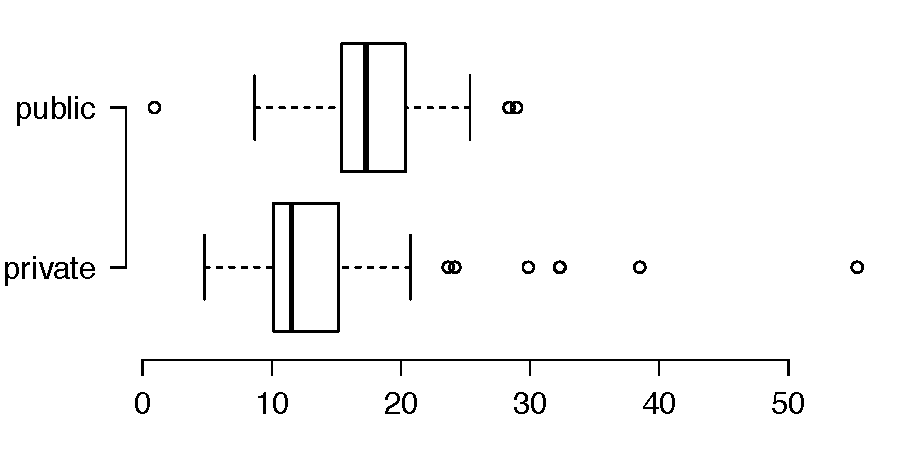
\includegraphics[width=0.4\textwidth]{ratio/ratio_box}
\end{center}
\end{multicols}

\begin{enumerate}

\item We would like to test if there is a \emph{difference} between the average student-to-faculty ratio between public and private four-year colleges using a randomization test. What are the hypotheses?

\item Fill in the blanks below for the appropriate set up for this test:

\begin{doublespace}
We write the student-to-faculty ratio of each public and private college in this sample on a total of \rule{2cm}{0.5pt} index cards. Then, we shuffle these cards and split them into two groups: one group of size \rule{2cm}{0.5pt} representing public colleges, and another group of size \rule{2cm}{0.5pt} representing private colleges. We calculate the difference between the average student-to-faculty ratios in the public and private colleges ($\bar{x}_{public} - \bar{x}_{private}$) and record this value. We repeat this many times to build a randomization distribution, which should be centered at \rule{2cm}{0.5pt} . Lastly, we calculate the p-value as the proportion of simulations where the simulated differences in means are \rule{2cm}{0.5pt}.
\end{doublespace}

\item The dot plot below is created using 100 simulations. What is the p-value?

\begin{center}
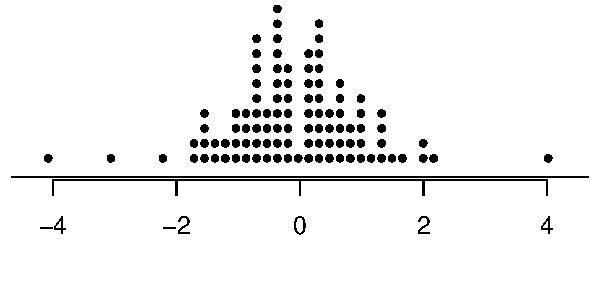
\includegraphics[width=0.6\textwidth]{ratio/rand_dist}
\end{center}

\item Based on the p-value, do these data provide convincing evidence to suggest that the student-to-faculty ratio in public four-year colleges is different than that of private four-year  colleges.

\end{enumerate}

\end{document}